\chapter{Fundamentação Teórica}\label{fundamentacao}

\section{Manutenção de Software}\label{manutencao}
A manutenção de software é qualquer alteração em um sistema de software após a implantação em seu ambiente de operação. Todo software passa por mudanças para adaptar-se a outro sistema operacional, mudanças de requisitos, ou simplesmente correção de funcionalidades. Atualmente as empresas estão tendo uma maior atenção ao processo de manutenção de software segundo \apud{pigoski1997,polo2002}{figueiredo2005}. Este custo não se restringe a apenas termos financeiros, bem como retrabalho. O esforço de retrabalho ocorre pelo fato da maioria das equipes de manutenção não estarem relacionadas com a equipe de desenvolvimento e pelo fato da pouca atenção com a documentação do software, com o decorrer do tempo evoluções no software são realizadas e a documentação não é devidamente atualizada \cite{sergio2005}.

\subsection{Tipos de Manutenção}
Como citado anteriormente todo software passa por mudanças, e essas mudanças sendo realizadas após a entrega do software caracterizam a atividade de manutenção. "Um software não se desgasta como peças de um equipamento, mas se deteriora no sentido de os objetivos de suas funcionalidades cada vez menos se adequarem ao ambiente externo" \space  \cite[p.~33]{matheus2007}.

Os tipos de manutenção definidas são: \apud{lientz1980}{matheus2007} \textit{corretivas}, \textit{adaptativa} e \textit{perfectivas} 
\subsubsection{Manutenção Corretiva}
Manutenções corretivas visam corrigir defeitos funcionais, onde uma determinada funcionalidade do sistema se comporta de maneira diferentes da especificada para aquela funcionalidade.
\apudonline{pfleeger2001}{matheus2007} relata um problema de impressão de um relatório, em que as linhas que eram impressas por cada folha eram maiores do que foi especificado, sobrepondo as informações das outras linhas. O problema foi identificado como uma falha de driver da impressora, e foi preciso alterar o menu de impressão para adicionar um novo parâmetro, este que iria referenciar o número de linhas que seria impresso.
\subsubsection{Manutenção Adaptativa}
As manutenções do tipo adaptativa retratam a alteração do software de modo a adaptá-lo a um novo ambiente de execução. Por exemplo, alterar o sistema devido a uma nova lei, que força o sistema a se \textbf{adaptar} ao ambiente externo \apudonline{pfleeger2001}{matheus2007} aborda uma situação onde havia um Sistema de  Gerência de Banco de Dados (SGBD) que foi atualizado, e as rotinas de acesso ao disco também foram alteradas, necessitando de uma parâmetro adicional. Este tipo de manutenção tem como característica não a correção de defeitos, até por que não existia, mas adaptá-lo ao novo ambiente de operação.
\subsubsection{Manutenção Perfectiva}
Manutenções perfectivas tem como objetivo adicionar funcionalidades ao sistemas, seja para obter um \textit{business value} maior ao produto de software, para competir com um software concorrente no mercado, ou simplesmente para atender uma solicitação de usuário. Este processo de mundaça é realizado mediante uma avaliação prévia  do sistema, que visa avaliar se a arquitetura do sistema suporta as novas funcionalidades sem degradá-la.
\subsection{Custos de Manutenção}
Para toda empresa, quanto menos custos melhor, mas o cenário atual nos diz que os maiores custos em produto de software estão na fase de manutenção\apud{pigoski1997,polo2002}{figueiredo2005}
e não alterar o software de maneira rápida o suficiente pode gerar grandes prejuízos. Os altos custo relacionados a manutenção estão inerentes a manutenção em si, esta atividade lida com diversos problemas com má documentação do software a ser mantido, e a imprevisibilidade, não saber em que estado o sistema foi construído, sobre que técnicas, padrões, metodologias, etc. 
\subsection{Documentação de Manutenção}

\subsection{Plano de Gerenciamento de Configuração}
O Plano de Gerenciamento de Configuração (PGC) descreve todas as atividades de configuração e mudança que serão realizadas durante o projeto. Um conjunto de atividades, responsabilidades, ferramentas, recursos e etc. A gerência de configuração tem como objetivo garantir a integridade dos itens de configuração, que são qualquer artefato que esteja sob custódia da Gerência de Configuração, através do versionamento, da identificação, controlando mudanças e acesso. 
\section{Gerência de Configuração}
A gerência de configuração é a área da engenharia de software responsável pela evolução do software. Ela atua durante todo o ciclo de vida do produto de software e, por meio de técnicas, ferramentas e metodologias, visa garantir que as mudanças que irão ocorrer dentro do ciclo de vida do desenvolvimento do software sejam identificadas, avaliadas e comunicada a todos os envolvidos através de ferramentas que auxiliam neste processo de evolução.
Portanto "o propósito do processo de Gerência de Configuração é estabelecer e manter a integridade de todos os produtos de trabalho de um processo ou projeto e disponibilizá-la a todos os envolvidos"\space\cite{mpsbr}.
\subsection{Sistema de Controle de Versão}
Um sistema de controle de versão: "	[...] combina procedimentos e ferramentas para gerenciar diferentes versões de objetos de configurações que são criadas durante o processo de engenharia de software" \cite[p.~927]{pressman2010}.
Atualmente, o uso de sistema de controle de versão se tornou comum nas empresas de grande e pequeno porte. Tais ferramentas permitem que se tenha o controle de diferentes versões de arquivos que estão submetidos ao versionamento, recuperação de versões antigas, visualizar alterações realizadas em arquivos e saber por quem e quando o arquivo foi alterado. Através de comandos (i.e.,\textit{check-in},\textit{check-out}) os usuários conseguem se comunicar com o repositório a fim de obter os artefatos ali armazenados \cite{gleiph2011}. Em situações especais faz-se necessário que os desenvolvedores trabalhem em una linha diferente da original chamada de \textit{mainline}, geralmente essa situação ocorre quando tem-se como objetivo consertar bugs de versões anteriores do repositório, nesse caso um \textit{branch}, uma ramificação na linha de desenvolvimento do controle de versão que permite o trabalho em paralelo sobre o mesmo repositório.
\begin{figure}[tbh]
\centering
\caption[Branch no Sistema de Controle de Versão]{Branch no Sistema de Controle de Versão}
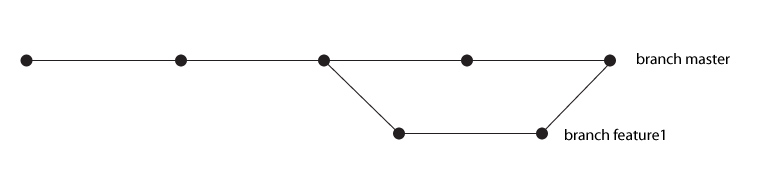
\includegraphics[width=0.7\linewidth]{./images/branch}
\label{fig:Branch}
\legend {\fontsize{10}{12}\selectfont {Fonte: \citeonline{tableless2012}}}
\end{figure}
A figura \autoref{fig:Branch} demonstra a criação de um \textit{branch} paralelo a linha de desenvolvimento principal chamada de branch feature1 e branch master respectivamente, posteriormente ocorre a integração das ações realizar no \textit{branch feature1} é incorporado ao \textit{branch master}.
\subsubsection{Sistema de Controle de Versão Local}
Um sistema de controle de versão local	armazenam todas as informações de um arquivo submetido ao versionamento na máquina local, guardando diferentes versões daquele arquivo localmente como demonstrado na figura \autoref{fig:SCVLocal}.
\begin{figure}[tbh]
\centering
\caption[Sistema de Controle de Versão Local]{Sistema de Controle de Versão Local}
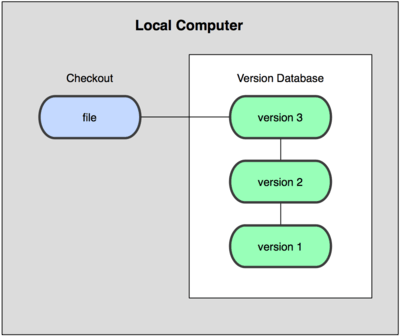
\includegraphics[width=0.5\linewidth]{./images/scvlocal}
\label{fig:SCVLocal}
\legend {\fontsize{10}{12}\selectfont {Fonte:\cite{git}}}
\end{figure}
\subsubsection{Sistema de Controle de Versão Centralizado} Sistema de controle de versão centralizado como o nome diz possuem um único servidor centralizado, como o \textit{subversion} \footnote{http://subversion.apache.org}, \textit{perforce} \footnote{http://www.perforce.com}, este tipo de padrão de SCV mantém em seu único servidor todos os arquivos versionados. Para cada comando de comunicação realizado nos arquivos versionados, uma requisição deverá ser feita, podendo gerar lentidão ou deixar o servidor fora de funcionamento.
\begin{figure}[tbh]
\centering
\caption[Sistema de Controle de Versão Centralizado]{Sistema de Controle de Versão Centralizado}
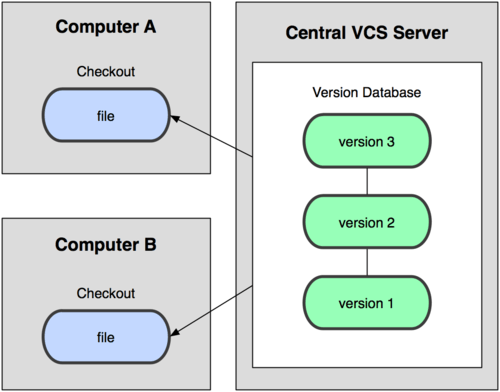
\includegraphics[width=0.5\linewidth]{./images/scvcentral}
\label{fig:SCVCentral}
\legend {\fontsize{10}{12}\selectfont {Fonte: \citeonline{git}}}
\end{figure}
No exemplo acima dois desenvolvedores trabalhando em máquinas diferentes realizam a comunicação com o servidor central para obter o artefato de trabalho.	
\subsubsection{Sistema de Controle de Versão Distribuído}Os sistemas de controle de versão distribuído possuem um servidor central onde os arquivos são submetidos a versionamento, entretanto cada desenvolvedor possui em sua máquina de trabalho as versões que estavam no servidor, tornando cada \textit{workstation} um "servidor", portanto, caso ocorra um problema no servidor central, estes podem ser recuperados via \textit{workstation}, mantendo a integridade dos arquivos e evitando ser um ponto único de falha, como mostra a figura \autoref{fig:SCVDistribuido}:
\begin{figure}[tbh]
\centering
\caption[Sistema de Controle de Versão Distribuído]{Sistema de Controle de Versão Distribuído}
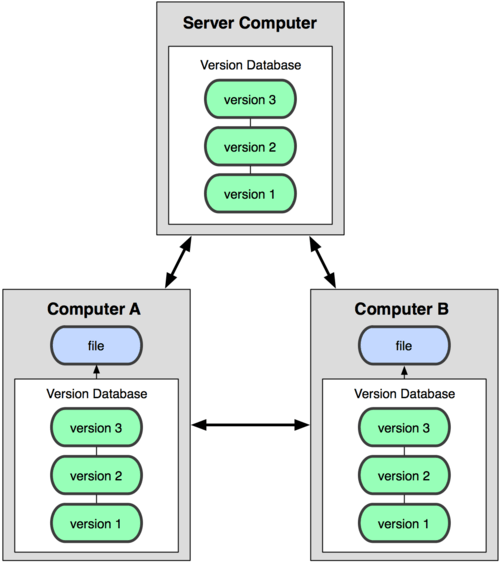
\includegraphics[width=0.5\linewidth]{./images/scvdist}
\label{fig:SCVDistribuido}
\legend {\fontsize{10}{12}\selectfont {Fonte: \citeonline{git}}}
\end{figure}
\subsection{Sistema de Controle de Mudança}
Todo software sofre mudanças, lidar com as mudanças é o papel da gerência de configuração, e para isso o gerente de configuração utiliza de um sistemas de controle de mudança. "O controle de mudança combina procedimentos humanos e ferramentas automatizadas para proporcionar um mecanismo de controle de mudança" \citeonline[p~.930]{pressman2010}. As mudanças devem ser avaliadas com cautela baseando-se, em seu custo benefício, uma combinação de esforço e \textit{business value}. A mudança tem início quando um "cliente" solicita a mudanças através de um formulário, conhecida com \textit{change request}. Nesse formulário é descrito os aspectos da mudança, após a solicitação ser realizada, esta deve ser avaliada, verificando se a mesma já foi solicitada, ou corrigida em caso de \textit{bugs}. Após a mudança ser validada, uma equipe de desenvolvedores e avaliam os impactos que esta mudança têm sobre o sistema, verificando custo/benefício e esforço de realização \cite{sommerville2011}. Posterior a essa análise, a mudança será avaliada por um comitê de controle de mudança (CCB) que avaliará o impacto da perspectiva do negócio, o que decidirá se esta mudança será revisada, aprovada ou reprovada. Alguns sistemas que fornecem este controle sobre as mudança são: \textit{redmine \footnote{http://www.redmine.org}, GitHub \footnote{http://www.github.com} Jira \footnote{https://www.atlassian.com/software/jira}}
\subsection{Auditoria de Configuração}
"Uma auditoria de configuração de software complementa a revisão técnica formal ao avaliar um objeto de configuração quanto às características que geralmente não são consideradas durante a revisão"\space\citeonline[p~.934]{pressman2010}. Ela tem como objetivo garantir que mesmo com as mudanças realizadas a qualidade foi mantida. As auditorias se dividem em dois tipos: auditorias funcionais e auditorias físicas, a auditoria funcional baseia-se em verificar se os itens de configuração estão devidamente atualizados e se as práticas e padrões foram realizados da maneira correta, enquanto a auditoria funcional, busca verificar os aspectos lógicos dos itens de configuração.
\subsection{Ferramentas de Build}
As ferramentas de build tem como objetivo automatizar processos repetitivos, aumentando a produtividade e facilitando o trabalho do desenvolvedor. Através da definição de uma rotina, ou conjunto de comandos, o desenvolvedor informa a ferramenta que tipo de processo ele deseja automatizar, pode ser desde compilar e testar uma classe, como dropar e criar uma tabela nova no banco de dados, comprimir arquivos css e javascript, cabe ao desenvolvedor definir o escopo da automatização. Alguns exemplo deste tipo de ferramenta são: \textit{Ant, Grunt, Gulp, Maven}.


\begin{figure}[h]
\centering
\caption[Processo Lógico de uma Build]{Processo Lógico de uma Build}
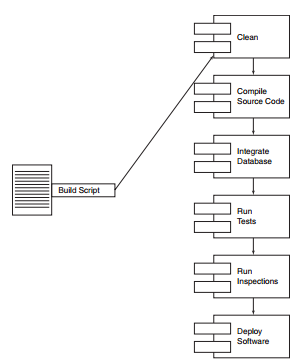
\includegraphics[width=0.7\linewidth]{./images/build}
\label{fig:build}
\legend {\fontsize{10}{12}\selectfont {Fonte: \citeonline{paul2007}}}
\end{figure}
Na figura \autoref{fig:build} um script foi definido para realizar as seguintes funções, será realizado um clean no projeto, compilará o código fonte, integrará com o banco de dados, executará testes e inspeções no código e por fim irá dar o \textit{deploy} da aplicação.


%\subsection{Ferramentas de Integração Contínua}

\section{Integração Contínua}\label{integracaocont}
\begin{OnehalfSpace}
A integração contínua tem como objetivo identificar erros o mais rápido possível, ela permite que alterações efetuadas e integradas aos repositórios dos sistemas de controle de versão (SCV) sejam posteriormente verificadas e caso erros ocorram, este serão notificados imediatamente ao autor da alteração.
Entende-se Integração Contínua como:
\end{OnehalfSpace}

\begin{citacao}
"[...] uma prática de desenvolvimento de software onde os membros de um time integram seu trabalho frequentemente, geralmente cada pessoa integra pelo menos diariamente – podendo haver múltiplas integrações por dia. Cada integração é verificada por uma build automatizada (incluindo testes) para detectar erros de integração o mais rápido possível. Muitos times acham que essa abordagem leva a uma significante redução nos problemas de integração e permite que um time desenvolva software coeso mais rapidamente." \citeonline[tradução nossa]{fowler2000}
\end{citacao}

\begin{figure}[tbh]
\centering
\caption[Ambiente de Integração Contínua]{Ambiente de Integração Contínua}
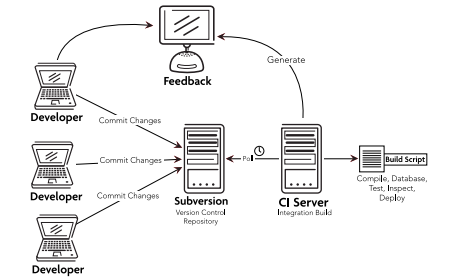
\includegraphics[width=0.8\linewidth]{./images/CI}
\label{fig:CI}
\legend {\fontsize{10}{12}\selectfont Fonte: \citeonline{paul2005}}
\end{figure}

A figura \autoref{fig:CI} descreve um ambiente em que um servidor de integração contínua é utilizado. Existem três ambientes de trabalho distintos formado por três desenvolvedores que obtiveram uma cópia do projeto do repositório do SCV para trabalharem em suas \textit{workstation}, durante o trabalho alterações foram realizadas e commitadas ao repositório central, após a inserção junto ao repositório o servidor de integração contínua verifica as alterações e executa uma build de integração,caso exista um problema com a build e esta quebre, o responsável pela alteração será informado sobre a quebra e terá como objetivo consertar a build.

As principais vantagens em utilizar um servidor de integração contínua segundo \citeonline[p.~29]{paul2007} são:

\begin{itemize}
\item Redução de Riscos.
\item Redução de processos manuais repetitivos.
\item Permitir melhor visibilidade do projeto.
\item Estabelecer uma maior confiança no produto do time de desenvolvimento.
\end{itemize}

%\subsection{Integração Contínua e a Redução de Riscos}
%Os Riscos em produtos de software estão diretamente relacionados. Segundo \citeonline[p~.48]{paul2007} se você consegue reduzir certos riscos no software, você pode melhorar a qualidade do software.
\subsection{Builds Automatizadas}
Builds são rotinas de execução definidas com o objetivo de reduzir processos repetitivos. Durante o processo de desenvolvimento de um software muitas ações tendem a serem repetidas por parte dos desenvolvedores, utilizar o tempo para a realização  de atividades que poderiam ser automatizadas, de forma manual, reduz a produtividade e preocupações com melhorias devido ao tempo "apertado". Somando-se a isso, uma build garante que tudo que está nela definido será executado, evitando assim, que determinada ação seja esquecida, ou caso um novo membro entre na equipe uma explicação do que ele deve fazer, ou não esquecer de fazer, não faz-se necessário.

\subsection{Integração Contínua Manual}
Na IC manual o processo de integração é realizado individualmente, possibilitando que 
apenas um desenvolvedor realize check-in no repositório durante o intervalo de integração \citeonline{gleiph2011}. Este tipo de abordagem como permite que apenas uma pessoa realize o \textit{check-in}, as integrações serão contínuas e seguidas e não paralelas, este tipo de abordagem garante uma maior confiabilidade das integrações, pois segue um padrão de integração, os itens do repositório possuem maior consistência e a garantia da estrutura do repositório é mantida \cite{gleiph2011}.

\subsection{Integração Contínua Automatizada}
A integração contínua automatizada é auxiliada pelo uso de um servidor de integração contínua, que obtém do controle de versão as alterações realizadas e executada sua build privada afim de verificar possíveis erros gerados por essas modificações. Ver \autoref{integracaocont} \autoref{fig:CI} 
\begin{citacao}
IC Automática possui a vantagem de ser escalável 
e,  deste  modo,  oferecer  maior  suporte  ao  trabalho  colaborativo.  Com  a  utilização  de 
Servidores  de  IC,  a  responsabilidade  de  realizar  construções  da  integração  é  retirada  dos desenvolvedores. Portanto, os desenvolvedores podem realizar  check-in  sem a necessidade de 
conquistar a vez de integrar. Esse fator é fundamental para que os  check-ins  continuem sendo 
verificados  sem  a  necessidade  de  um desenvolvedor  realizar  a  construção  e identificar 
problemas, resultando na eliminação do gargalo humano. \citeonline[p~.54]{gleiph2011}. 
\end{citacao}


%\subsection{Tipos de Build}
%\subsubsection{Builds Privadas}
%\subsubsection{Build de Integração}
%\subsubsection{Builds de Release}
%\subsubsection{Mecanismos de Build}
%\subsubsection{Builds Engatilhadas}